
\chapter{The Experiment}

\section{Large Hadron Collider}

The Large Hadron Collider (LHC) has a radius of approximately 27 kilometers. As of this writing, it is the largest machine ever constructed. The initial purpose of the LHC was to discover the Higgs boson.

\section{Compact Muon Solenoid}

The Compact Muon Solenoid (CMS) is a general-purpose particle detector located at Point-5 of the LHC. 

\centerline{
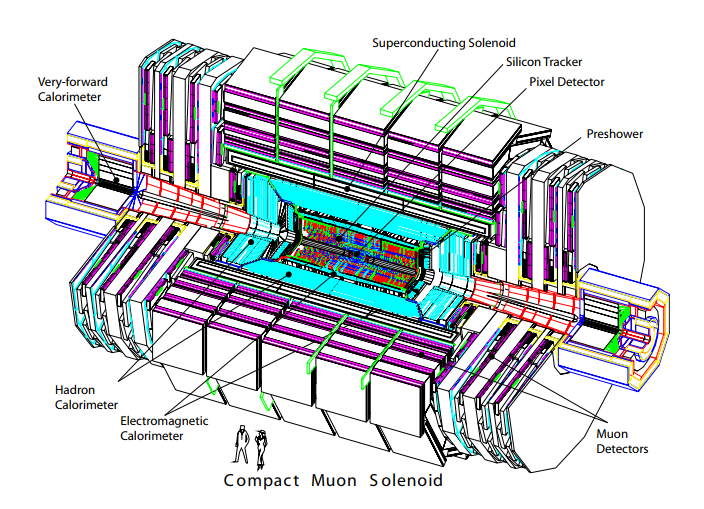
\includegraphics[width=5in]{Chapter3/importfigs/fromCMS_DesignPaper_perspective.png}
}

\subsection{Inner Tracker}

The tracker measures the momentum of charged particles via their trajectory through a homogenous magnetic field. The tracker consists of two units, the pixel tracker and the strip tracker, both of which are made of silicon. A charged particle causes an electrical signal when passing through a silicon pixel or silicon microstrip. CMS reconstructs these electrical signals, taken at specific points of position and time, into tracks. These tracks are accurate to the 10 micrometers. 

\subsubsection{Pixel Tracker}

Every silicon-pixel has a corresponding readout chip. The readout chips are soldered through the bump-bonding method. The readout chip amplifies signals from the pixel.

The pixel tracker is precise enough to distinguish the vertices of tracks originating from short-lived particles, such as bottomonia. 

\subsubsection{Strip Tracker}

\subsection{Electromagnetic Calorimeter}

The Electromagnetic Calorimeter (ECAL)

\subsection{Hadronic Calorimeter}

The Hadronic Calorimeter (HCAL) has such a large acceptance that it can indirectly observe non-interacting particles such as neutrinos.


\subsubsection{Hadronic Forward Calorimeters}

The Hadronic Forward Calorimeters (HF) absorbs the greatest portion of energy from collisions. As such it is designed for maximum radiative resistance.

\subsection{Muon Detector}

\subsection{Zero Degree Calorimeter}

\subsection{Luminosity}

One of the most important quantities measured by CMS is luminosity. Luminosity is necessary to convert the number of events detected, for a given channel, into a collision cross-section. Collision cross-sections are among the primary observables predicted by theoretical physics, specifically quantum field theory.

\subsubsection{van de Meer Scanning}

\subsection{Triggering}

CMS reconstruct events faster than they can be stored on hard-drives. To account for this phenomena -- pile-up -- CMS uses a two tiered triggering system. L1 triggers are always online, and for those events that pass the L1 triggers, the High Level Triggers (HLTs) will select which events are stored as data.